\chapter{Methods}

\section{Expanding the Wright-Fisher Model}
The simplest form of our model is based on the classic Wright-Fisher [3][4] and Stepping-Stone [5] models which describe evolution and migration, respectively. The model describes the allele frequency in a population of N individuals grouped into discrete demes, or subpopulations, connected by migration (Figure \ref{fig:schematic}). 

\begin{figure}
    \centering
    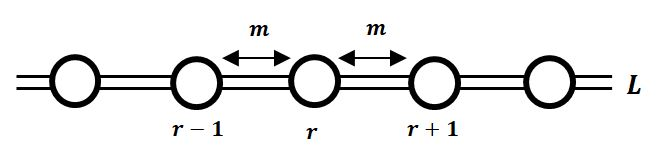
\includegraphics[scale=0.8]{img/model_schematic.JPG}
    \caption{This schematic represents the geographic structure for the model in one dimension. Circles represent demes which are indexed by integer $r$. There are $L$ many demes connected to nearest neighbors via a symmetric migration rate $m$.}
    \label{fig:schematic}
\end{figure}
	

The model simplifies the system by modeling a single genetic locus with two alleles. The allele frequency in each deme, $f_r$, evolves due to four forces:


\begin{enumerate}
    \item \textbf{Mutation} changes one allele to another at rate $\mu$;
    \item
\end{enumerate}
(1)  (2) Natural selection reduces the frequency of the deleterious allele at rate s; (3) Genetic drift introduces random noise in a finite population at rate 1/N, where N is the population size; (4) Migration reduces the allele frequency differences between neighboring demes at rate m. The change in allele frequency due to these forces is described by the stochastic differential equation:

$$
df_r=[μ(1-2f_r )-sf_r (1-f_r )]dt+√((f_r (1-f_r ))/N) dB_(t,r)+m[f_(r-1)+f_(r+1)-2f_r ]dt
$$

While these models have been studied extensively [14][15][16], most work has been focused on neutral evolution. Including non-neutral natural selection and the effect of sampling expands upon previous studies and enables novel conclusions.
Using this equation, the equilibrium distribution of allele frequencies across all demes can be calculated. In this project, the model describes the sampling process by choosing individuals from demes at random according to a sampling distribution. Given the population parameters and sampling probability distribution, the expected number of sampled individuals with the focal allele is calculated.




\subsection{The neutral Wright-Fisher model}

\subsection{Incorporating selection}

\subsection{Simulating a spatial environment}

\section{Principal Components Analysis}

\section{SLiM and computational resources used}
